
%%%%%%%%%%%%%%%%%%%%%%%%%%%%%%%%%%%%%%%%%%%%%%%%%%%%%%%%%%%%%%%%%%%%%%%%%%%%%%%
%
%  EGSnrc beamdp manual
%  Copyright (C) 2015 National Research Council Canada
%
%  This file is part of EGSnrc.
%
%  EGSnrc is free software: you can redistribute it and/or modify it under
%  the terms of the GNU Affero General Public License as published by the
%  Free Software Foundation, either version 3 of the License, or (at your
%  option) any later version.
%
%  EGSnrc is distributed in the hope that it will be useful, but WITHOUT ANY
%  WARRANTY; without even the implied warranty of MERCHANTABILITY or FITNESS
%  FOR A PARTICULAR PURPOSE.  See the GNU Affero General Public License for
%  more details.
%
%  You should have received a copy of the GNU Affero General Public License
%  along with EGSnrc. If not, see <http://www.gnu.org/licenses/>.
%
%%%%%%%%%%%%%%%%%%%%%%%%%%%%%%%%%%%%%%%%%%%%%%%%%%%%%%%%%%%%%%%%%%%%%%%%%%%%%%%
%
%  Authors:         Charlie Ma, 1995
%                   Dave Rogers, 1995
%
%  Contributors:    Andrew Booth
%                   Joanne Treurniet
%                   Blake Walters
%                   Iwan Kawrakow
%
%%%%%%%%%%%%%%%%%%%%%%%%%%%%%%%%%%%%%%%%%%%%%%%%%%%%%%%%%%%%%%%%%%%%%%%%%%%%%%%


\documentclass[12pt,twoside]{article}
\setlength{\textwidth}{6.5in}
\setlength{\textheight}{9.3in}
\setlength{\oddsidemargin}{0.0in}
\setlength{\evensidemargin}{0.0in}
\setlength{\topmargin}{-0.6in}
\setlength{\parindent}{1.5em}
\setlength{\topsep}{0ex}
\setlength{\itemsep}{0ex}

\newcommand{\Co}{$^{60}$Co}
\newcommand{\parsp}{~\hspace*{1.5em}}
\setlength{\parskip}{0.1in}
\setlength{\baselineskip}{0.4in}
\newcommand{\head}[1]{\begin{center}\begin{Large}{\bf #1}
                                              \end{Large}\end{center}}
\newcommand{\cen}[1]{\begin{center} #1 \end{center}                   }
\newcommand{\etal}{{\em et.al.}}
\newcommand{\etc}{{\em etc}}
\newcommand{\eg}{{\em e.g.}}
\newcommand{\ie}{{\em i.e.}}

\usepackage{graphicx}
\usepackage{html}
\usepackage{fancyhdr}
\renewcommand{\footrulewidth}{0.4pt}
\renewcommand{\headrulewidth}{0.4pt}

\lhead[{\sffamily \thepage~}]{{\sf NRCC Report PIRS-0509(C)revA}}
\rhead[{\sf BEAMDP Users Manual}]{{\sffamily ~\thepage}}
\rfoot{{{\sf \rightmark}}}
\lfoot[{{\sf \leftmark}}]{{\small Last edited $Date: 2013/03/29 15:20:16 $
}}
\cfoot{}

\renewcommand{\refname}{}




\begin{document}

\thispagestyle{empty}

\begin{htmlonly}
For information about the authors and/or institutions involved with this
work, use the links provided in the author list.
\begin{rawhtml}
<br><br>
\end{rawhtml}

\begin{rawhtml}
<br><br>
\end{rawhtml}

\begin{rawhtml}
<br><br>
\end{rawhtml}

Use the Up button to get back to this page from within the document.
\begin{rawhtml}
<BR> <HR> <P>
\end{rawhtml}
\copyright
Copyright 2015, National Research Council of Canada Ottawa
\begin{rawhtml}
<BR> <HR> <P>
\end{rawhtml}
\end{htmlonly}

%\markright{BEAMDP Users Manual~~~~~~last edited 30 Sep 1999
%~~~~printed \today \hfill page~~}
%\markboth{BEAMDP Users Manual}{NRCC Report PIRS-0509(C)}

%\setcounter{page}{1}
\pagestyle{empty}

\title{BEAMDP Users Manual}
\author{ C.-M. Ma and D.W.O. Rogers \\
Ionizing Radiation Standards\\
National Research Council of Canada,
Ottawa\\
}

\date{Printed: \today \\
NRCC Report PIRS-0509(C)revA
\begin{latexonly}
\end{latexonly}
}
\maketitle

\pagenumbering{arabic}
\setlength{\parindent}{0em}

\begin{center}
\begin{Large}
{\bf Abstract}
\end{Large}
\end{center}
This user's manual describes the structure, function and usage of the BEAMDP (BEAM Data Processor) computer program. BEAMDP
is developed for the OMEGA (Ottawa Madison Electron Gamma Algorithm) project. BEAMDP can be used to analyze the phase-space parameters of a clinical electron beam generated using BEAMnrc and to derive the data required by a multiple-source model for representation and reconstruction of the electron beam for use in Monte Carlo radiotherapy treatment planning.

\newpage
\mbox{}	%blank behind title page
\newpage
\setcounter{page}{1}
\pagestyle{fancy}

\tableofcontents

\newpage

%\pagestyle{myheadings}

\section{Introduction}
BEAMDP (BEAM Data Processor) is an interactive program, developed for the OMEGA
(Ottawa Madison Electron Gamma Algorithm) project. BEAMDP helps the
BEAMnrc\cite{Ro95,Ro04a} users to analyze the electron beam data obtained by the
Monte Carlo simulation of the coupled transport of photons and electrons in a
clinical accelerator and to derive the data required by the simplified
sub-source models of these electron beams for use in Monte Carlo radiotherapy
treatment planning\cite{MR04b,Ma95c}.

\vspace{0.2cm}
When running BEAMDP, a user is given the following options:


\begin{enumerate}
\item to analyze a phase-space data file for beam characterization models;
\item to derive fluence vs position from a phase-space data file;
\item to derive energy fluence vs position from a phase-space data file;
\item to derive spectral distributions from a phase-space data file;
\item to derive an energy fluence distribution from a phase-space data file;
\item to derive mean energy distributions from a phase-space data file;
\item to derive angular distributions from a phase-space data file;
\item to derive distributions for {\tt ZLAST} from a phase-space data file;
\item to derive the distribution of particle weights from the phase-space data
file;
\item to combine two phase-space files into one;
\item to list the parameters of phase-space particles on the screen.
\end{enumerate}

\noindent
Options (1) through (10) are described in greater details in the report ``BEAMDP as a General-Purpose Utility'' written by Ma and Rogers\cite{MR04b}. The details of beam representation and reconstruction using simplified sub-source models can be found in report ``Beam Characterization: a Multiple-Source Model'' by Ma and Rogers\cite{Ma95c}. This user's manual describes the structure, function and usage of the BEAMDP (BEAM Data Processor) computer program for analysis of  the BEAM phase-space data and generation of source parameter files required for the multiple-source model for representation and reconstruction of electron beams for use in Monte Carlo radiotherapy treatment planning.


\section{Description of BEAMDP}
\subsection{Files related to BEAMDP}

The following files are required in order to run BEAMDP:
\begin{description}
\item [{\tt Makefile}] Located in {\tt \$OMEGA\_HOME/progs/beamdp}.
This directs the compilation of BEAMDP.  The files that are concatenated
to create {\tt mortjob.mortran} (the file that is actually MORTRAN/Fortran
compiled) are defined in the {\tt SOURCES} variable.  This file also
sources the configuration files {\tt \$HEN\_HOUSE/specs/config.conf}
and \\
{\tt \$HEN\_HOUSE/specs/beamnrc.spec} for definitions of environment
variables.
\item [{\tt beamdp.mortran}] Located in {\tt \$OMEGA\_HOME/progs/beamdp}.
This is the MORTRAN source file
\item [{\tt filename.egsphsp\#}] phase-space file generated by BEAM (\# can be 1, 2 or 3)
\item [{\tt filename}] source parameter file for beam characterization models
\item [{\tt filename}] BEAMDP output file for use by {\tt xmgr/xvgr} plotting package
\end{description}

\subsection{Structure and Function of {\tt beamdp.mortran}}

BEAMDP consists of a MAIN routine and 8 subroutines. The following sections describe the structures of these routines and how they work.

\subsubsection{The Main Routine}
BEAMDP is mainly designed to help the BEAMnrc users to analyze the beam data
obtained by the Monte Carlo simulation of clinical electron beams and to derive the data required by the simplified sub-source models of these beams for use in Monte Carlo radiotherapy treatment planning. Once a user has chosen the option for beam model analysis subroutine {\tt beamdp1} will be called and more operations can be chosen within this subroutine.

BEAMDP can also be used as a general-purpose  BEAM utility program to derive energy, planar fluence, mean energy, angular distributions, \etc., from an existing phase-space data file generated by BEAM. These operations are performed mainly in the main routine and it loops within the main until the user requests to quit the program.

\subsubsection{Subroutine {\tt readname}}
This is a simple subroutine which inquires the user for a file name.

\subsubsection{Subroutine {\tt openfile}}
This subroutine is called from several subroutines as many features in
BEAMDP require inputs from and/or outputs to phase-space files.

In general, phase-space files generated by BEAM can be classified into two
categories: {\tt MODE0} files and {\tt MODE2} files. Both files are
directly-accessible, unformatted and of fixed record length. Each record
in a {\tt MODE0} file contains 7 variables while in a {\tt MODE2} file it
contains 8 variables (see the BEAMnrc Users Manual\cite{Ro04a}).

Subroutine {\tt openfile} will first try to open a file as a {\tt MODE0}
file. If it fails, it will then try to open it as a {\tt MODE2} file. If it
fails again, it returns with a ``directory/file not found''  message.
\subsubsection{Subroutine {\tt add\_files}} One of the features of BEAMDP
is to combine two phase-space files into one. This is useful if a BEAM run
is being split among different machines and the user wishes to add the
phase-space data together at a later stage. Subroutine {\tt add\_files}
performs this operation.

The user is required to input two file names. The data in the first file will be added to the second file. The second file can then be renamed  the user wishes to do so.

\subsubsection{Subroutine {\tt read\_data}} Subroutine {\tt read\_data} is
called by the main routine. {\tt read\_data} performs the phase-space data
reading and parameter translation. {\tt read\_data} bins the phase-space
particles according to their charge, energy, position, angle, and/or {\tt
LATCH} settings. This gives the energy spectrum, particle planar fluence
distribution, mean energy and angular distributions, \etc. When requested,
{\tt read\_data} also processes and lists the phase-space parameters on
the screen.

\subsubsection{Subroutine {\tt beamdp1}} This is the main subroutine in
{\tt beamdp.mortran} for beam characterization analysis. It has the
following functions: (1) reading sub-source geometry information; (2)
processing phase-space data; (3) generating sub-source parameter data; (4)
plotting energy or planar fluence distributions for the sub-sources using
the {\tt xvgr/xmgr} plotting package; and (5) creating source parameter
input files.

Subroutine {\tt beamdp1} is called from the main routine and it will loop
the operations mentioned above inside the subroutine and quit until it is
requested.  \subsubsection{Subroutine {\tt read\_phsp}} Subroutine {\tt
read\_phsp} is called from {\tt beamdp1}. {\tt read\_phsp} analyzes the
phase-space data and scores the energy spectra, planar fluence
distributions, and angular distributions for the beam characterization
models. Phase-space particles are grouped into sub-sources based on their
charge and origin. Particles not scored due to spatial restrictions or
charge, or wrong {\tt LATCH} settings are counted  and then reported in
{\tt beamdp1}.  \subsubsection{Subroutine {\tt xvgrplot}} {\tt xvgrplot }
was written by Andrew Booth as a general-purpose utility routine for data
output in a format for use by {\tt xvgr/xmgr} plotting package, and later
modified to include necessary features for use by BEAMDP. {\tt xvgrplot}
creates a file containing the plotting data supplied by the user and a
minimum set of parameters required by {\tt xvgr/xmgr}. A user can pass on
the following information through the subroutine call (each call outputs
data for one curve and one data file can contain several curves):

\begin{description} \item [~~~~$X(NPTS)$]  array of x values to be
plotted, top of bin if histogram \item [~~~~$Y(NPTS)$]  corresponding
array of y values to be plotted \item [~~~~$ERRY(NPTS)$]  array of errors
in y for the plot, non-zero values of ERRY mean the graph is of type
XY-DY, otherwise, of type XY \item [~~~~$NPTS$]  number of data points for
the curve \item [~~~~$CURVENUM$]  curve number in a graph (starting with
0) \item [~~~~$SERIESTITLE$]  string ($<$60 characters), legend for a
curve in the graph \item [~~~~$GRAPHTITLE$]   string ($<$60 characters),
title for the graph \item [~~~~$SUBTITLE$]  string ($<$60 characters),
subtitle for the graph (default to phase-space file name where the data is
derived) \item [~~~~$TYPE$]  graph type: 0 for normal point plot, 1 for
histogram \item [~~~~$UNITNUM$]  logical unit number, specifying where the
data is to be written \item [~~~~$XTITLE$]  string ($<$60 characters),
title for x-axis \item [~~~~$YTITLE$]  string ($<$60 characters), title
for y-axis \item [~~~~$HISTXMIN$]  the value of the lowest x-bin, only for
histogram \end{description}


\subsubsection{Subroutine {\tt xvgr\_script}}
Subroutine {\tt xvgr\_script}  is used to generate a Unix script file
(called {\tt xmgr\_script}) which is automatically called from within
BEAMDP to plot data using XMGR/XVGR.  Note that this subroutine is only
useful if you are running on a Linux/Unix platform.

\subsection{Compiling and running BEAMDP}

BEAMDP is normally installed and compiled as part of the OMEGA/BEAM
installation (See the BEAMnrc Manual\cite{Ro04a} for installation
instructions).

To compile BEAMDP separately, go into directory {\tt \$OMEGA\_HOME/progs/beamdp}
and type:
\begin{verbatim}
make
\end{verbatim}
The files specified in the {\tt SOURCE} variable in {\tt Makefile}
will then be concatenated together to create {\tt mortjob.mortran}, which
is then MORTRAN/Fortran compiled.  In addition to {\tt mortjob.mortran},
compilation will also leave the files {\tt beamdp\_config.mortlst}
(listing from the MORTRAN compilation) and
{\tt beamdp\_config.f} (Fortran code) in the
{\tt \$OMEGA\_HOME/progs/beamdp} directory.  The executable, {\tt beamdp*},
will be left in {\tt \$HEN\_HOUSE/bin/config}, where {\tt config} is the
name of the configuration you are running on (eg {\tt gcc}, {\tt win2k}).

To run BEAMDP from the command line, type:
\begin{verbatim}
beamdp
\end{verbatim}
Note that you must
have {\tt \$HEN\_HOUSE/bin/config}, where {\tt config} is the name
of the configuration you are running on, as part of your {\tt \$PATH}
environment variable.
BEAMDP will prompt you for input.  To create a source model, select
option (0).

Running BEAMDP is much easier using the BEAMDP GUI\cite{Tr04}.  To start the GUI in
a Linux/Unix window, type:
\begin{verbatim}
beamdp_gui
\end{verbatim}
Note that you must have sourced the Unix script
{\tt \$HEN\_HOUSE/scripts/beamnrc\_cshrc\_additions} (or
{\tt \$HEN\_HOUSE/scripts/beamnrc\_bashrc\_additions}) in your
{\tt .cshrc} (or {\tt .bashrc}) file.  See the BEAMnrc Users Manual\cite{Ro04a}
for more information about these scripts.  To start the GUI in a Windows
environment, double click on the GUI icon (or on the name
{\tt beamdp\_gui} if you have entered directory
{\tt \$OMEGA\_HOME/progs/gui/beamdp} using Windows Explorer).

Once in the GUI, you must select the option to
``Process data for beam characterization models''.

\subsection{Source Parameter File}

\subsubsection{Introduction}
A source parameter file contains the information about a multiple sub-source model. A source parameter file consists of two parts: (1) information about source geometry, energy range, field size, \etc., of a multiple-source model, and (2) the energy, planar fluence, angular distributions of the sub-source, \etc.
A previously generated source parameter file  can be used by BEAMDP as a source geometry input file in order to process new BEAM phase-space data. Only the first part of the source parameter file will be read by BEAMDP for this purpose. When a source parameter file is used by BEAM and other EGS4 usercodes in the beam re-construction process all the information stored in the file is required.

\subsubsection{Contents of a Source Parameter File}
The following parameters are included in a source parameter file:
\begin{description}
\item [~~~~$1.~~ INFO$] information about the accelerator and the beam energy, field size, SSD, \etc. ($<$80 characters)
\item [~~~~$2. ~~N_{source}$] number of sub-sources in the multiple-source model
\item [~~~~$3. ~~TYPE,CHARGE,I_{bit}$] source type (applicator, collimator, planar source, point source), particle charge (-1: electron, 0: photon, 1: positron), bit number of LATCH corresponding to this sub-source (\ie, an accelerator component)
\item [~~~~$4. ~~SOURCE DIMENSIONS$] source dimensions, orientation, \etc.

(Input 3 and 4  $N_{source}$ times)

\item [~~~~$5. ~~N_{bin},E_{min},E_{max}$] number of energy bins for the spectrum, minimum kinetic energy, maximum kinetic energy of the phase-space particles in file
\item [~~~~$6. ~~FIELD TYPE$] field type for planar fluence scoring (circular, square, rectangular)
\item [~~~~$7. ~~FIELD DIMENSIONS$] dimensions of treatment field and scoring field (scoring field should be larger than the treatment field)
\item [~~~~$8. ~~FILENAME$] name of phase-space file to be processed by BEAMDP ($<$80 characters)

\item [~~~~$9. ~~I_{source}$] sub-source number
\item [~~~~$10. ~~TYPE,CHARGE,I_{bit}$] same as 2 above
\item [~~~~$11. ~~SOURCE DIMENSIONS$] same as 3 above
\item [~~~~$12. ~~RELATIVE INTENSITY$] relative source intensity
\item [~~~~$13. ~~N_{bin},E_{min},E_{max}$] same as 6 above
\item [~~~~$14. ~~E(N_{bin})_{in}$] energy distribution inside the treatment field
\item [~~~~$15. ~~E(N_{bin})_{out}$] energy distribution outside the treatment field
\item [~~~~$16. ~~FIELD TYPE$] same as 6 above
\item [~~~~$17. ~~FIELD DIMENSIONS$] same as 7 above
\item [~~~~$18. ~~\phi(N_{bin})$] planar fluence distribution for the sub-source
\item [~~~~$19. ~~A(N_{bin}),B(N_{bin})$] parameters required to correct for the variation of planar fluence within a spatial bin (only for square field type)

(Input 10 through 19 $N_{source}$ times)

\item [~~~~$20. ~~ANGLE(N_{bin})$] angular distribution of direct electrons used to correct for the effect of charged particles scattering in air

\end{description}

\section{Multiple-Subsource Model}
\subsection{Introduction}

The idea behind the model-based beam characterization is that particles from different parts of a accelerator may be treated as they are from different sub-sources. This is supported by the fact that particles from different components of an accelerator have different energy, angular and spatial distributions. The particles from the same component, however, have very similar characteristics, in terms of energy range and incident directions, which are almost independent of their positions on the scoring plane\cite{Ma95c}.

A variety of sub-sources have been developed with respect to the components in an accelerator. A point source corresponds to the particles coming from the vacuum window without hitting any of the beam confining components, such as collimators or applicators. Parallel bars and annular sources are used to simulate collimators. Rectangular sources are used for the applicators. Photons, electrons and positrons are simulated as separate sources.

The origin of a particle is classified using the information recorded in {\tt LATCH},
which contains the region numbers where the particle has been to, has
interacted, or was created if it is a secondary particle. The origin of a
photon is considered to be the region where it is created or last
scattered; for a charged particle, the origin is the last non-air region
it has been to before crossing the scoring plane.

Each sub-source has its own spectral and planar fluence distributions derived from the simulated phase-space data (the size of a source parameter file is about 100 Kb). By sampling the particle position on the sub-source and on the phantom surface, the correlation between the particle position and incident angle is naturally retained. For charged particles, a small perturbation of the incident direction is sampled to correct for the effect of charged particles scattering in the air.

This multiple-source model has been implemented in BEAMnrc, DOSXYZnrc and other EGSnrc
user codes. The use of beam models does not provide any time savings for the dose calculations. It is possible, however, to model a simulated beam with 10\% or less particles than required for Monte Carlo simulations, without adversely affecting the accuracy of the dose calculation. This represents a CPU time saving for the treatment head simulation of over a factor of 10 as well as considerable savings in data storage requirements (the size of a typical phase-space data file from a ``standard'' Monte Carlo run is 100 Mb or more).
More importantly, the beam model study improved our understanding of the clinical electron beams which may lead to better accelerator design and beam applications.


\subsection{Subsource Models for Commonly-Used Accelerators}
\subsubsection{Aperture Applicator}
Aperture applicators are modelled as surfaces on the (x,y) plane with zero thickness. This is a good approximation of more recent applicator designs.

The dimensions of the applicator opening (\ie., the aperture) should be exactly the same as that of the applicator being modelled. The particles are considered to be non-uniform on the surface, with more coming from the edges of the opening.
It is not necessary, however, that the applicator model have the same outer dimensions as those of the
applicator. The dimensions of a charged particle sub-source can be considered to be equivalent to inner opening dimensions + a 0.5 - 2.0 cm margin. However, for the lowest applicator (closest to the patient) the actual applicator dimensions should be used as electrons created by bremsstrahlung photons can also reach the phantom surface. For bremsstrahlung photons, the outer dimensions of the sub-sources should correspond to those of an area actually ``exposed'' to
the electron beam; most of the electrons are stopped by the applicator but the x-rays created by them can reach the scoring plane (contaminant photons). In most cases, the actual outer dimensions can be used for the photon sources. The distance from the sub-source to the phantom surface can be calculated from the mid-point of the applicator thickness to the phantom surface.
The following variables specify the applicator dimensions (see Fig.~\ref{source1}):


\begin{description}
\item [~~~~$Z_{min}$] distance (in cm) from the sub-source to the scoring plane
\item [~~~~$X-$] minimum x coordinate (cm) for the opening of the applicator
\item [~~~~$X+$] maximum x coordinate (cm) for the opening of the applicator
\item [~~~~$Y-$] minimum y coordinate (cm) for the opening of the applicator
\item [~~~~$Y+$] maximum y coordinate (cm) for the opening of the applicator
\item [~~~~$|X|_{max}$] maximum absolute x coordinate (cm) for the applicator (the outer dimension)
\item [~~~~$|Y|_{max}$] maximum absolute y coordinate (cm) for the applicator (the outer dimension)
\end{description}

\begin{figure}[htbp]
\begin{center}
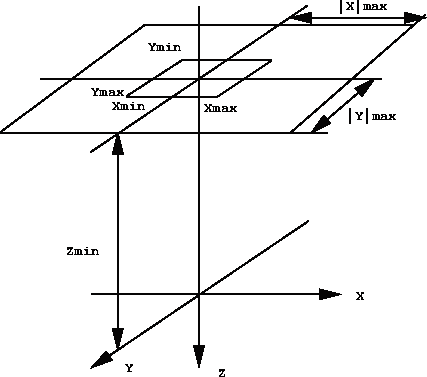
\includegraphics[height=15cm]{figures/source1}
\caption[]
{Schematic diagram of an aperture applicator source. }
\label{source1}
\end{center}
\end{figure}

\subsubsection{Tubular Applicator}
Tubular applicators are modelled as tubular surfaces expanded in the z-direction. This is an approximation of  the ``old'' design such as that used in Philips SL75-20 accelerator. A tubular applicator can also be simulated using a series of stacked aperture applicators.

The source dimensions are similar to those for aperture applicators except that both the distances from the bottom and the top of the sub-source to the phantom surface are required.

The following variables specify the tubular applicator dimensions(see Fig.~\ref{source11}):


\begin{description}
\item [~~~~$Z_{min}$] distance (in cm) from the bottom of the sub-source to the scoring plane
\item [~~~~$Z_{max}$] distance (in cm) from the top of the sub-source to the scoring plane
\item [~~~~$X-$] minimum x coordinate (cm) for the opening of the applicator
\item [~~~~$X+$] maximum x coordinate (cm) for the opening of the applicator
\item [~~~~$Y-$] minimum y coordinate (cm) for the opening of the applicator
\item [~~~~$Y+$] maximum y coordinate (cm) for the opening of the applicator
\item [~~~~$|X|_{max}$] maximum absolute x coordinate (cm) for the applicator (the outer dimension)
\item [~~~~$|Y|_{max}$] maximum absolute y coordinate (cm) for the applicator (the outer dimension)
\end{description}
\begin{figure}[htbp]
\begin{center}
\leavevmode
\mbox{}\hspace{0cm}
\vspace*{5cm}
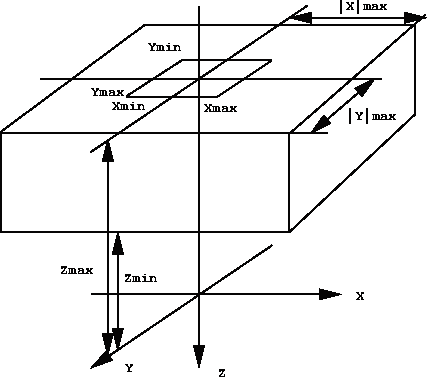
\includegraphics[height=15cm]{figures/source11}
\caption[] {Schematic diagram of a tubular applicator source. }
\label{source11}
\end{center}
\end{figure}
\subsubsection{Collimator jaw}
Collimator jaws are modelled as parallel-bars with zero height. The orientation of the collimator bars can be either along the x- or y-axis. The particles are considered to be from the surface non-uniformly, with more coming from the edges of the opening. The distance from the sub-source to the phantom surface can be calculated from the mid-point of the collimator thickness to the phantom surface. The dimensions of the sub-source are the same as those of the actual collimator.

The following variables specify this source(see Fig.~\ref{source2}):

\begin{description}
\item [~~~~$Z_{min}$] distance (in cm) from the sub-source to the scoring plane
\item [~~~~$X-$] minimum x coordinate (cm) for the opening of the applicator
\item [~~~~$X+$] maximum x coordinate (cm) for the opening of the applicator
\item [~~~~$Y-$] minimum y coordinate (cm) for the opening of the applicator
\item [~~~~$Y+$] maximum y coordinate (cm) for the opening of the applicator
\item [~~~~$|X|_{max}$] maximum absolute x coordinate (cm) for the applicator (the outer dimension
\item [~~~~$|Y|_{max}$] maximum absolute y coordinate (cm) for the applicator (the outer dimension
\item [~~~~$Orient$] jaw orientation (0: bars along x-axis, 1: along y-axis)
\end{description}
\begin{figure}[htbp]
\begin{center}
\leavevmode
\mbox{}\hspace{0cm}
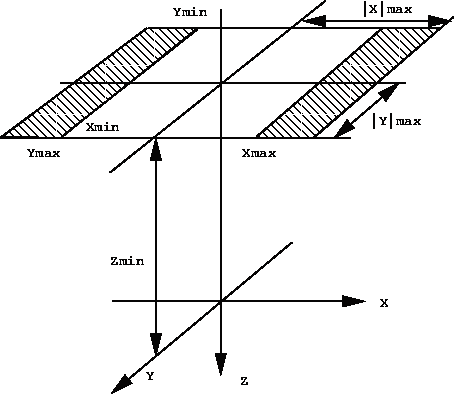
\includegraphics[height=15cm]{figures/source2}
\caption[]
{Schematic diagram of a source for collimator jaws. }
\label{source2}
\end{center}
\end{figure}
\subsubsection{Ring, Cone and Point Source}
Primary collimators are usually ring- or cone-shaped; they are modelled as a ring with zero height. The dimensions of the sub-source are the same as that of the actual ring or cone and the distance from the sub-source to the phantom surface can be calculated from the mid-point of the ring/cone thickness to the phantom surface. The particles are considered to be from the surface non-uniformly, with more coming from the edges of the opening.
When the radius of this sub-source is set to zero the sub-source becomes a point source. For a point source the user is asked to input the source surface distance, $Z_{min}$ (see below), which can be a dummy or default value (say, 100 cm) as $Z_{min}$ will be re-evaluated by the BEAMDP program anyway.

The following variables specify this source(see Fig.~\ref{source3}):

\begin{description}
\item [~~~~$Z_{min}$] distance (in cm) from the sub-source to the scoring plane
\item [~~~~$R_{min}$] radius of the inner opening of the ring or cone (= 0 for point source)
\item [~~~~$R_{max}$] outer radius of the ring or cone (= 0 for point source)
\end{description}

\begin{figure}[htbp]
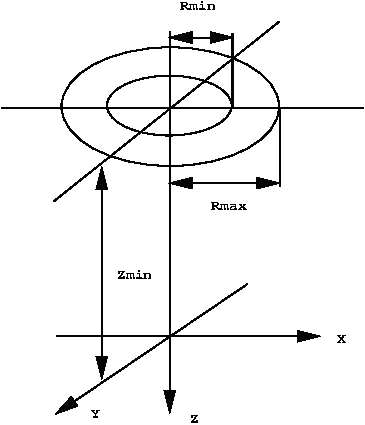
\includegraphics[height=15cm]{figures/source3}
\caption[]
{Schematic diagram of an annular source for ring, cone or point source. }
\label{source3}
\end{figure}

Note that for a virtual point source the source-surface distance, SSD$_{vir}$ (= $Z_{min}$ input by the user) will be re-evaluated using a method similar to the ``pin-hole'' method\cite{Ma95c}. This requires the user to input in the next line the radius of a thin ring region within the treatment field:

\begin{description}
\item [~~~~$R_{ring}$] outer radius of a  ring for virtual SSD analysis
\end{description}

The ring width is equal to $R_{ring}$/40 (i.e., the inner radius = $R_{ring}$ - $R_{ring}$/40), which will be set by the program.

\subsubsection{Planar Sources}
Scattering foils, mirrors and monitoring ionization chambers are modelled
as either rectangular or circular planar sources. The dimensions of the
sub-source are the same as that of an area actually ``exposed'' to the
electron beam but with zero thickness. Particles are sampled uniformly on
the source surface. The distance from the sub-source to the phantom
surface can be calculated from the mid-point of the component thickness to
the phantom surface.

Planar sub-sources are mainly used for bremsstrahlung photons as they are
created directly in these components and their origins are well-defined.
For charged particles, however, planar sub-sources can generally be
replaced by a virtual point source.

{\bf Rectangular Planar Source}

The following variables specify a rectangular planar source(see Fig.~\ref{source4}):
\begin{description}
\item [~~~~$Z_{min}$] distance (in cm) from the sub-source to the scoring plane
\item [~~~~$X-$] minimum x coordinate (cm) of the planar source
\item [~~~~$X+$] maximum x coordinate (cm) of the planar source
\item [~~~~$Y-$] minimum y coordinate (cm) of the planar source
\item [~~~~$Y+$] maximum y coordinate (cm) of the planar source

\end{description}
\begin{figure}[htbp]
\begin{center}
\leavevmode
\mbox{}\hspace{0cm}
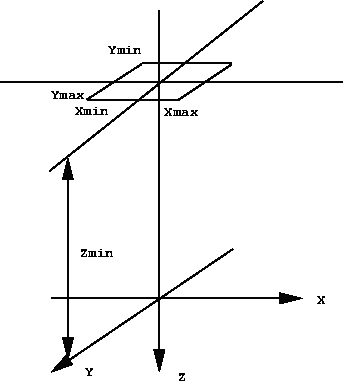
\includegraphics[height=15cm]{figures/source4}
\caption[]
{Schematic diagram of a rectangular planar source. }
\label{source4}
\end{center}
\end{figure}

{\bf Circular Planar Source}

The following variables specify a circular planar  source(see Fig.~\ref{source5}):

\begin{description}
\item [~~~~$Z_{min}$] distance (in cm) from the sub-source to the scoring plane
\item [~~~~$R$] radius of the planar source

\end{description}

\begin{figure}[htbp]
\begin{center}
\leavevmode
\mbox{}\hspace{0cm}
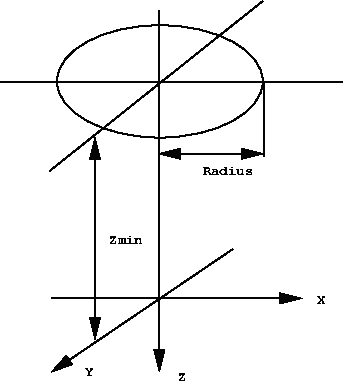
\includegraphics[height=15cm]{figures/source5}
\caption[]
{Schematic diagram of a circular planar source. }
\label{source5}
\end{center}
\end{figure}
\subsection{Energy Spectrum}
\subsubsection{Introduction}
BEAMDP analyzes the BEAM phase-space data and generates two energy distributions: one for particles inside the treatment field and the other for particles outside the treatment field. This is based on the fact that the mean particle energy varies significantly around the treatment edge but remains fairly constant well-inside or well-outside the treatment field (away from the field edges). The dimensions of the treatment field are given by the user (see inputs for field dimensions).

The maximum number of energy bins allowed is 200 but this can be changed
by modifying the {\tt beamdp.mortran} program (variable {\tt \$NB}). Since
electron depth-dose curves are sensitive to the electron incident energy,
especially to the energies of the direct electrons, which usually have a
very narrow peak, it is suggested that 0.1 MeV bin width be used for an
energy distribution.

\subsubsection{Variables Set on Input}
The user is required to input the following variables for the analysis of the energy distributions:
\begin{description}
\item [~~~~$N_{bin}$] number of bins for an energy distribution (1-200)
\item [~~~~$E_{min}$] minimum kinetic energy of phase-space particles in file
\item [~~~~$E_{max}$] maximum kinetic energy of phase-space particles in file
\end{description}


\subsection{Planar Fluence}
\subsubsection{Introduction}
Each sub-source has its own particle planar fluence distribution, which can be scored in either a circular field with annular bins of equal area, a square field with square rings of equal area, or a rectangular field with rectangular regions of equal area. The user also needs to input the dimensions of the treatment field, which will only be used for energy spectra scoring.
Note that, once chosen,  all the sub-sources will use the same field type for their planar fluence distributions.

\subsubsection{Circular Field}
The circular planar fluence scoring field (see Fig.~\ref{field}a) is
centred on the z-axis. It has $N_{bin}$ annular bins of equal area. Equal
bin area ensures less statistical fluctuation of planar fluence from bin
to bin. Clearly, circular fields are good for beams confined by circular
linac components such as those scattered by scattering foils, monitoring
chamber, mirror, and confined by ring- or cone-collimators. Fields formed
by rectangular linac components such as jaws and applicators are not
suitable for this field type. The user also needs to input the dimensions
of the treatment field which will be used by energy spectrum scoring as
described in the previous section. The treatment field should be smaller
than the planar fluence scoring field. \\

The following variables are required for the planar fluence
distribution(see Fig.~\ref{field}a):  \begin{description} \item
[~~~~$N_{bin}$] number of bins for a planar fluence distribution (1-200)
\item [~~~~$R_{treat}$] radius of the treatment field \item
[~~~~$R_{score}$] radius of the scoring field used in the BEAM simulation
\end{description} \begin{figure}[htbp] \begin{center} \leavevmode
\mbox{}
\hspace{0cm}
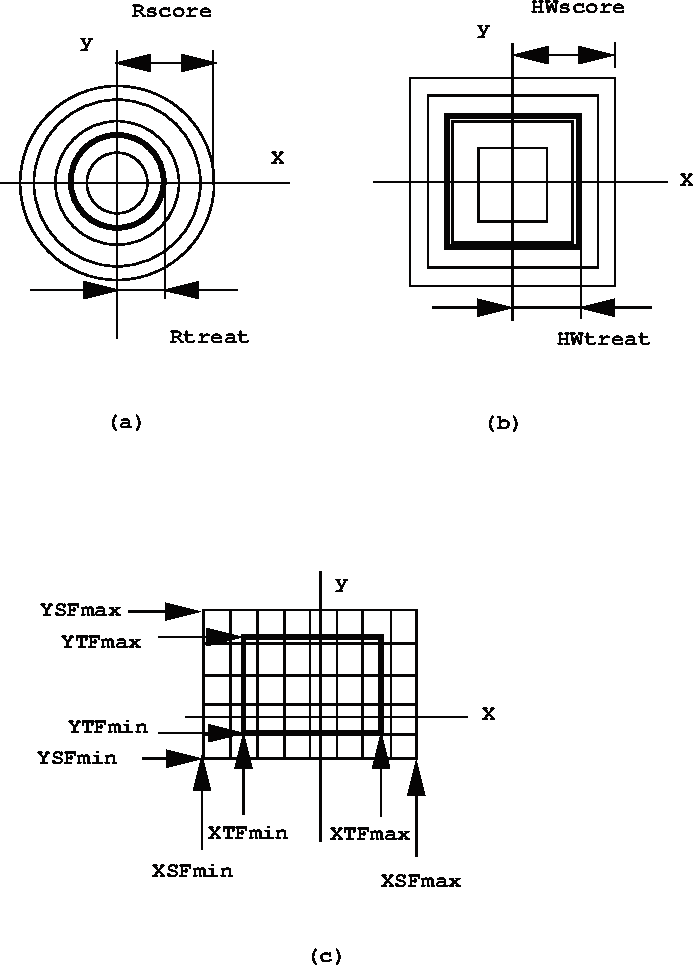
\includegraphics[height=21cm]{figures/field}
\caption[]
{Schematic diagram of field types: (a) a circular field, (b) a square
field, and (c) a rectangular field. } \label{field} \end{center}
\end{figure}

\subsubsection{Square Field} The square planar fluence
scoring field (see Fig.~\ref{field}b) is also centred on the z-axis. The
field is defined by its half-width (x-/y-directions), and divided into
$N_{bin}$  square rings of equal area.  The user is also required to input
the dimensions of the treatment field for energy spectrum scoring, which
should be within the planar fluence scoring field.\\

The following variables are required for the planar fluence distribution in a square field (see Fig.~\ref{field}b):
\begin{description}
\item [~~~~$N_{bin}$] number of bins for a planar fluence distribution (1-200)
\item [~~~~$HW_{treat}$] half-width of the treatment field
\item [~~~~$HW_{score}$] half-width of the scoring field used in the BEAM simulation
\end{description}

\subsubsection{Rectangular Field}

This option allows the user to set-up asymmetric and/or off-axis fields. The rectangular field (see Fig.~\ref{field}c) is divided into $N_{bin}$ x $N_{bin}$ equal rectangular areas to record the planar fluence. The following variables are required for the planar fluence distribution in a rectangular field:
\begin{description}
\item [~~~~$N_{bin}$] number of bins for a planar fluence distribution (1-200)
\item [~~~~$XSF-$] minimum x coordinate of the rectangular scoring field
\item [~~~~$XSF+$] maximum x coordinate of the rectangular scoring field
\item [~~~~$YSF-$] minimum y coordinate of the rectangular scoring field
\item [~~~~$YSF+$] maximum y coordinate of the rectangular scoring field
\end{description}
In the next line the user should input the dimensions of the treatment field (see Fig.~\ref{field}c).
\begin{description}
\item [~~~~$XTF-$] minimum x coordinate of the treatment field
\item [~~~~$XTF+$] maximum x coordinate of the treatment field
\item [~~~~$YTF-$] minimum y coordinate of the treatment field
\item [~~~~$YTF+$] maximum y coordinate of the treatment field
\end{description}

\subsubsection{Circular Field with Energy Spectra Defined in Multiple Radial
               Bins}

Similar to the circular field option, this option allows the user to define
a scoring field radius, $R_{score}$, and number
of radial bins, $N_{bin}$, within the scoring field.  Hoewever, in this option,
energy spectra are defined in each of the radial bins, as opposed to the
regular circular field option in which energy spectra are only defined inside
the treatment field and outside it.  Thus, with this option, the user does
not need to input a treatment field radius.

\subsection{Angular Distribution}
To correct for the effect of the electron multiple-scattering in air, the
angular distribution of the electron beam going through 100 cm air is
required by the re-construction procedure in order to produce an angular
perturbation around the already chosen electron incident direction. BEAMDP
analyzes the simulated beam phase-space data and scores the angular
spread  of the ``direct'' electrons within a circle of 1 cm radius (\ie,
the angle between the particle incident direction and the z-axis,
$\theta$). This angular spread is considered to be a good approximation of
that for a pencil beam of electrons of the same energies going through an
air slab of thickness equal to the $SSD_{direct}$ of the ``direct''
electrons. This angular distribution is also stored in the source
parameter file for beam re-construction.  No user input is required while
running BEAMDP.

\subsection{{\tt LATCH} Settings}
For beam characterization models we suggest using {\tt LATCH } option 3
for the BEAM simulations (See the BEAMnrc Users Manual\cite{Ro04a}).
In this option, bits 1 to 23 of {\tt LATCH} record where a charged particle
has been or where a photon has interacted and bits 24 - 28 are used to record
the region of origin of a secondary particle.  {\tt LATCH} bits are associated
with
regions/components of an accelerator using the {\tt IREGION\_TO\_BIT}
input parameter.  In bits 1 - 23, the actual bit specified by
{\tt IREGION\_TO\_BIT} is set (note that this means that the maximum
possible value of {\tt IREGION\_TO\_BIT} is 23), and in bits 24 - 28, the value of
{\tt IREGION\_TO\_BIT} is stored using the 5 available bits.

We suggest using one value of
{\tt IREGION\_TO\_BIT} for at
least one accelerator component.  Note that bit 23 is the default and
is associated with all air within the accelerator.  Thus we do not
recommend using {\tt IREGION\_TO\_BIT}=23 for any accelerator components, and,
in fact, BEAMDP won't let you input {\tt LATCH} bit 23 for any sub-source.

In BEAMDP, the single
{\tt LATCH} bit input for a sub-source should correspond to the
{\tt IREGION\_TO\_BIT} value for the accelerator component(s) comprising
the sub-source.  BEAMDP then determines the origin of a particle, and further
calculates the relative source
intensity, energy spectrum, planar fluence distribution, \etc., for the
sub-source based on this {\tt LATCH} bit setting.  The selected {\tt LATCH}
bit must be $\leq$ 22.  As stated
above, bit 23 is generally associated with the air in the accelerator and,
thus, cannot be assigned to any sub-source.  If the input
{\tt LATCH} bit is $\leq$ 0, then the user is saying that particles
from this sub-source have NONE of bits 1 - 22 set.  This option is
generally used for virtual point sources of photons that have been created
in the target, but that do not interact anywhere in the accelerator
(including the target).

After the user has input the charge and {\tt LATCH} bit number for all the
sub-sources, BEAMDP will re-number the sub-sources based on the distance from
the sub-source to the scoring plane (or phantom/patient surface), starting with
 the nearest sub-source as number 1. During the analysis of phase-space data,
the {\tt LATCH} bit corresponding to the nearest sub-source is checked first.
If it is set the particle is considered to be from this sub-source, otherwise,
the {\tt LATCH} bit corresponding to the second nearest sub-source is checked,
and so on.

In the BEAM simulation it is convenient to allocate {\tt LATCH} bit 1 to the
nearest component
(usually an applicator), bit 2 to the second nearest component, and so on.
Thus, the particles coming from the applicators and collimators
will be classified first. The rest (mainly direct electrons) can then be
modelled using a virtual point source. Components such as scattering foils,
monitoring chamber and mirror can be allocated to the same bit.
This makes it easier to classify the direct electrons and the photons
from the virtual point source.

\section{Running BEAMDP for Beam Model Analysis}

For BEAM data analysis for beam characterization models,  a BEAMDP run mainly consists of three parts: (1) geometry inputs for simplified sub-sources (data can be either typed in through keyboard or read in from an existing source parameter file ), (2) BEAM data analysis (the phase-space data is processed according to the input information and requirements from the user), and (3) data outputs for simplified source models or for {\it xmgr/xvgr} plots.

The program provides two levels of prompts for information, one for ``experienced'' users and one for ``new'' users. Detailed descriptions of the required input and range of acceptable values are given to the new users. After the first run through the program the shorter, less informative prompts are provided, to the ``experienced'' users. However, at any time the user may obtain additional information about any of the inputs by typing ``?'', or providing an unacceptable value.\\

The user can choose from the following beam characterization operations:

\begin{description}
\item [~~~~Option 0] generate new source parameter file and then analyze phase-space data
\item [~~~~Option 1] modify an existing source parameter file only
\item [~~~~Option 2] analyze phase-space data using an existing source parameter file
\item [~~~~Option 3] plot energy spectra or planar fluence distributions based on the information stored in an existing source parameter file

\end{description}

The following sections describe how to perform these operations.

\subsection{Input Source Parameters and Analyze Phase-Space Data}
This is a frequently used operation.

To input the source geometry and other information about the electron beam, one can type in the data interactively according to the on-line instructions, or use a reference source parameter input file and modify it as needed. This will create a new source parameter input file for a multiple sub-source model.

To analyze the phase-space data, one needs to supply a phase-space file
name. BEAMDP will automatically detect the mode of a phase-space file and
open it accordingly. Although BEAMDP can read {\tt MODE2} files which also
include the {\tt ZLAST} variable, the current multiple-subsource model
does not require the information about the z-position within an
accelerator component where the bremsstrahlung photons are created or last
interacted. BEAMDP classifies the phase-space particles into different
sub-sources and scores their energy and planar fluence distributions
according to which accelerator component they come from or last
interacted.

The user is asked to type in a file name for the source parameter output
file which will contain both the source geometry information and the
calculated energy and planar fluence distributions. This file can then be
used by BEAMnrc or other EGSnrc usercodes such as DOSXYZnrc for beam
re-construction. Good beam representation and reconstruction may be
obtained using a combination of sub-source models. It should be kept in
mind that a modelled beam can be very different from that represented by
the original phase-space data. Therefore, a modelled beam should be
carefully tested to ensure its accuracy and validity.

\subsection{Change Source Parameters in an Old Source File}
It is often convenient to change the parameters of a multiple-source
model. One can run BEAMDP interactively and change the source dimensions,
charge, field type, {\tt LATCH} settings, \etc., on line. It should be
noted that the number of sub-sources for a multiple-source model is
predetermined in the old source parameter file which cannot be changed  on
line. However, this parameter can be changed using a file editor. The
modified source parameter file can be used as a BEAM source parameter
input file for phase-space data analysis.

\subsection{Analyze Phase-Space Data Using an Old Source File}
Once a source parameter input file has been created one can run BEAMDP to
analyze the simulated phase-space data. The user will be asked whether to
change the information about the beam or the source model, to distinguish
the current file from any previous analysis. One can also input a
different file name to store the analyzed source parameters output  by
BEAMDP.  This file is called the source parameter output file, which can
be used directly for the beam re-construction process.

\subsection{Process an Old Source Parameter File for Graph Plotting}
BEAMDP allows the user to print out the energy and planar fluence
distributions stored in a source parameter file. For the energy spectra,
the user can choose from either inside or outside the treatment field and
for any number of sub-sources. For the planar fluence, the scoring field
type is already set up, \ie, circular, square or rectangular field. For a
rectangular field, the user inputs the orientation (0 for a distribution
along the x-axis and 1 for y-axis) and the bin number.  For a rectangular
field of 21 x 21 voxels centred at z-axis, for example, orientation = 0
and bin number = 21 will result in a planar fluence distribution varying
in the x-direction along the y$_{max}$ boundary.

Several energy or planar fluence distributions can be put into one data file (or plotted on one graph using {\tt xvgr/xmgr} within BEAMDP if requested). However, energy, planar fluence, or results for different field types should not be put in the same data file as the graph parameters may be mixed up.
\section{Examples}

\subsection{ A Sample BEAMDP Session}

\noindent
The following is a sample BEAMDP session on a Silicon Graphics machine. We select 3 sub-sources for a 18 MeV electron beam from a Varian Clinac 2100C accelerator. The BEAM phase-space data is stored in a file called {\tt vc21-18.egs4phsp1}. The BEAMDP output file is called {\tt sample.output} which can be used by BEAM or DOSXYZ for beam re-construction. It should be noted that {\tt sample.output}  is only a sample file because 3 sub-sources are not enough to re-construct the 18 MeV electron beam.

Note that although this example is somewhat dated, it is still a valid
illustration of command line input.

\begin{verbatim}
irs8> beamdp

 This is beamdp (SID 1.0 last edited 20/9/95)
 It takes an execute module and runs it on a(n) iris-R4x00.

 run beamdp.IRIX.exe

 Running BEADP, Version 1.0...
 -----------------------------------------------------------
 Type ? at any prompt for help

 BEAMDP (BEAM Data Processor) creates a source data input file
 for beam characterization models with information obtained
 from the user and derived from a full phase-space data file
 created by BEAM.

 This program can be used to derive planar fluence, spectrum,
 mean energy and angle distribution, \etc., from a phase-space
 file created by BEAM.

 If you are not familiar with this program, you can get an
 explanation before any input request. Otherwise, the prompts
 will be terse.

 However, you can get help by typing a ? to any prompt.

 Do you wish more detailed information about the file created
 by the program?   (y/n[Default])=> n


 Input a number for the operation required:
 ******************************************

 (0) - Process data for beam characterization models
 (1) - Derive planar fluence from ph-sp data
 (2) - Derive spectral distribution from ph-sp data
 (3) - Derive mean energy distribution from ph-sp data
 (4) - Derive angular distribution from ph-sp data
 (5) - Derive {\tt ZLAST} distribution from ph-sp data
 (6) - Combine two ph-sp files into one
 (7) - List parameters for a number of ph-sp particles
 (8) - Quit

 0

 Input a number to choose an option:
 ***********************************

 (0) - Input new source parameters & analyze new ph-sp data
 (1) - Only change parameters in an old source parameter file
 (2) - Process ph-sp data using an old source parameter file
 (3) - Plot graphs using data from a source parameter file
 (4) - Quit

 0

 Would you like to use an old source parameter file as a reference?
 (y/n[Default])=> n

 Name of the new source parameter file:
 sample.output

 Detailed information about the source:

 THE OLD INFORMATION WAS:

 (Return to keep the information, otherwise type in the new one):

 This is a sample BEAMDP file (VCl2100C 18 MeV,10x10cm field, 100cm SSD)

 Number of sub-sources:
 3

 INPUT PARAMETERS FOR SUB-SOURCE  1:

 SOURCE TYPE(1&11-appl,2-coll,3-ring,4-rect.plane,5-circ.plane),
 CHARGE OF PARTICLES (0-photons,-1-electrons,1-positrons),
 LATCH NUMBER FOR THE SUB-SOURCE DURING BEAM SIMULATION
 1,0,3

 Zmin, X-, X+, Y-, Y+, |x|max, |y|max (in cm) OF THE SOURCE:
 6.,-4.8,4.8,-4.8,4.8,7.,7.

 INPUT PARAMETERS FOR SUB-SOURCE  2:

 SOURCE TYPE(1&11-appl,2-coll,3-ring,4-rect.plane,5-circ.plane),
 CHARGE OF PARTICLES (0-photons,-1-electrons,1-positrons),
 LATCH NUMBER FOR THE SUB-SOURCE DURING BEAM SIMULATION
 2,-1,8

 Zmin,X-,X+,Y-,Y+,|x|max,|y|max(in cm),Orientation OF THE SOURCE
 (0-collimator bars along x-axis,1-along y-axis):
 72.,-2.,2.,-2.,2.,2.1,2.1,0

 INPUT PARAMETERS FOR SUB-SOURCE 3:

 SOURCE TYPE(1&11-appl,2-coll,3-ring,4-rect.plane,5-circ.plane),
 CHARGE OF PARTICLES (0-photons,-1-electrons,1-positrons),
 LATCH NUMBER FOR THE SUB-SOURCE DURING BEAM SIMULATION
 3,-1,11

 SSD, Rmin and Rmax OF THE SOURCE(=0 for point source):
 90.,0.,0.

 Radius(cm) of a ring region on the surface for SSD analysis:
 4.5

 Nbin, Emin, and Emax (in MeV, kinetic only) FOR THE SPECTRUM:
 168,0.189,21.

 FIELD TYPE (0-circular ring, 1-square ring, 2-rectangular):
 1

 Nbin, 1/2 TREATMENT FIELD WIDTH and 1/2 SCORING FIELD WIDTH:
 64,5.,10.

 The order of the sub-sources in terms of their distances to the
 scoring plane and their LATCH numbers:

   order     sub-source #         SSD           LATCH #       CHARGE

     1             1           	 6.000              3            0
     2             2            72.000              8           -1
     3             3            90.000             11           -1

 NAME OF FILE CONTAINING PHASE SPACE DATA (WITH EXT., < A80):
 /usr/people/cma/egs4/BEAM_VC18/vc21-18-new.egs4phsp1

 First, try to open it as a MODE0 file

 TOTAL NUMBER OF PARTICLES IN FILE       :   4389318
 TOTAL NUMBER OF PHOTONS                 :   3428931
 THE REST ARE ELECTRONS/POSITRONS.

 MAXIMUM  KINETIC ENERGY OF THE PARTICLES:    20.700 MeV
 MINIMUM  KINETIC ENERGY OF THE ELECTRONS:     0.189 MeV
 MINIMUM  KINETIC ENERGY OF THE PHOTONS  :     0.010 MeV

 BEGIN READING PH-SP DATA .....

 BEGIN SUMMARIZING THE PH-SP DATA.....

         INFORMATION ABOUT THE FULL PHASE SPACE DATA

 Read total    4389318 particles and ignored  0 multiple passer
 There were     953668 electrons with average energy     16.2051 MeV
 There were    3428931 photons with average energy        2.3931 MeV
 There were       6719 positrons with average energy      4.4343 MeV
 Maximum particle energy was                               20.700 MeV

              2119087  PARTICLES SCORED FOR ENERGY AND FLUENCE DISTRIBUTION
              2115323  PARTICLES IGNORED BECAUSE LATCH # WERE NOT SET
                    0  OF THEM ARE ELECTRONS
              2108604  OF THEM ARE PHOTONS, AN
                 6719  OF THEM ARE POSITRON
 ALSO          154908  PARTICLES NOT SCORED DUE TO OUT OF THE FIELD

 The virtual SSD for source   3 is   89.6 cm according to the full ph-sp data.

 BEGIN OUTPUTTING DATA.....

 SSD FOR SUB-SOURCE   3 HAS BEEN RE-SET FROM   90.0 cm TO   89.6 cm
 ACCORDING TO THE PHASE-SPACE DATA.

 WOULD YOU LIKE TO RUN THIS PROGRAM AGAIN?

 INPUT (1) TO CONTINUE OR (0) TO QUIT
 0

 BYE!

irs8>

\end{verbatim}

\subsection{A Sample BEAMDP Input File}
While running BEAMDP a user has the option to use a  reference source parameter file as a
BEAMDP input file to avoid inputting all the information required for the sub-sources interactively.
The BEAMDP input file can be generated either by running BEAMDP interactively or by writing a new BEAMDP input file or modifying an existing source parameter file using an editor. It is very convenient to modify an existing file and one has less chance to make a mistake. The following is a sample BEAMDP input file which can be generated by the interactive session given in the previous section by interrupting the program just before processing the phase-space data.

{\bf sample.input}
\begin{verbatim}
--------------------------------------
This is a sample BEAMDP file (VCl2100C 18 MeV,10x10cm field, 100cm SSD)
3
1  0  3
6.00000   -4.80000   4.80000   -4.80000   4.80000   7.00000   7.00000
2  -1  8
72.0000   -2.00000   2.00000   -2.00000   2.00000   2.10000   2.10000  0
3  -1  11
90.0000 0. 0.   4.50000
21  0.   21.0000
1
20    5.00000   10.00000
/usr/people/cma/egs4/BEAM_VC18/vc21-18.egs4phsp1
1
1  0  3
6.00000   -4.80000   4.80000   -4.80000   4.80000   7.00000   7.00000
0.  0.
21  0.  21.0000
0. 0. 0. 0. 0. 0. 0. 0. 0. 0. 0. 0. 0. 0. 0. 0. 0. 0. 0. 0. 0.
0. 0. 0. 0. 0. 0. 0. 0. 0. 0. 0. 0. 0. 0. 0. 0. 0. 0. 0. 0. 0.
1
20   10.00000
0. 0. 0. 0. 0. 0. 0. 0. 0. 0. 0. 0. 0. 0. 0. 0. 0. 0. 0. 0.
0. 0. 0. 0. 0. 0. 0. 0. 0. 0. 0. 0. 0. 0. 0. 0. 0. 0. 0. 0.
0. 0. 0. 0. 0. 0. 0. 0. 0. 0. 0. 0. 0. 0. 0. 0. 0. 0. 0. 0.
2
2  -1  8
72.0000  -2.00000   2.00000   -2.00000   2.00000   2.10000   2.10000  0
0.   0.
21  0.   21.0000
0. 0. 0. 0. 0. 0. 0. 0. 0. 0. 0. 0. 0. 0. 0. 0. 0. 0. 0. 0. 0.
0. 0. 0. 0. 0. 0. 0. 0. 0. 0. 0. 0. 0. 0. 0. 0. 0. 0. 0. 0. 0.
1
20   10.00000
0. 0. 0. 0. 0. 0. 0. 0. 0. 0. 0. 0. 0. 0. 0. 0. 0. 0. 0. 0.
0. 0. 0. 0. 0. 0. 0. 0. 0. 0. 0. 0. 0. 0. 0. 0. 0. 0. 0. 0.
0. 0. 0. 0. 0. 0. 0. 0. 0. 0. 0. 0. 0. 0. 0. 0. 0. 0. 0. 0.
3
3  -1  11
89.5719  0. 0.  4.50000
0.   0.
21  0.  21.0000
0. 0. 0. 0. 0. 0. 0. 0. 0. 0. 0. 0. 0. 0. 0. 0. 0. 0. 0. 0. 0.
0. 0. 0. 0. 0. 0. 0. 0. 0. 0. 0. 0. 0. 0. 0. 0. 0. 0. 0. 0. 0.
1
20   10.00000
0. 0. 0. 0. 0. 0. 0. 0. 0. 0. 0. 0. 0. 0. 0. 0. 0. 0. 0. 0.
0. 0. 0. 0. 0. 0. 0. 0. 0. 0. 0. 0. 0. 0. 0. 0. 0. 0. 0. 0.
0. 0. 0. 0. 0. 0. 0. 0. 0. 0. 0. 0. 0. 0. 0. 0. 0. 0. 0. 0.
0. 0. 0. 0. 0. 0. 0. 0. 0. 0. 0. 0. 0. 0. 0. 0. 0. 0. 0. 0.
0. 0. 0. 0. 0. 0. 0. 0. 0. 0. 0. 0. 0. 0. 0. 0. 0. 0. 0. 0.
0. 0. 0. 0. 0. 0. 0. 0. 0. 0. 0. 0. 0. 0. 0. 0. 0. 0. 0. 0.
0. 0. 0. 0. 0. 0. 0. 0. 0. 0. 0. 0. 0. 0. 0. 0. 0. 0. 0. 0.
0. 0. 0. 0. 0. 0. 0. 0. 0. 0.
(end of file)------------------------------------------
\end{verbatim}

(Note: Except for the first 12 lines, the rest will not be read by the code if this file is used as a BEAMDP reference input file and therefore are redundant if one is writing/editing the input file using an editor rather than by running BEAMDP.)

\subsection{A Sample BEAMDP Output File}
The following is a sample BEAMDP output file generated by the sample interactive session described previously. Compared with the sample BEAMDP input file the BEAMDP output file contains not only the information about the sub-source geometry but also the energy, planar fluence and angular distributions required for beam re-construction. For convenience, comments have been added at the end of lines to describe what they are.

{\bf sample.output}
\begin{verbatim}
--------------------------------------

This is a sample BEAMDP file (VCl2100C 18 MeV,10x10cm field, 100cm SSD)
3
1  0  3
6.00000   -4.80000    4.80000   -4.80000    4.80000    7.00000    7.00000
2  -1  8
72.0000   -2.00000    2.00000   -2.00000    2.00000    2.10000    2.10000  0
3  -1  11
89.5719  0. 0. ; SSD, $R_{inner}, R_{outer}$
21  0.   21.0000
1
20    5.00000   10.00000  0.
/usr/people/cma/egs4/BEAM_VC18/vc21-18.egs4phsp1
1;   sub-source 1 is an aperture applicator, photon source
1  0  3
6.00000   -4.80000    4.80000   -4.80000    4.80000    7.00000    7.00000
0.570536 89.5719;  relative source intensity, SSD for a virtual point source
21  0.   21.0000;  21 energy bins, range: 0 - 21 MeV
202778.   50082.0    23929.0    14252.0    9351.00    6579.00    4726.00
3477.00    2504.00    1991.00    1468.00    1051.00    733.000    522.000
418.000    220.000    112.000    52.0000    12.0000  0. 0.
474623.   152216.   78547.0    48773.0    33386.0    24114.0    17786.0
13584.0    10638.0    8013.00    6411.00    5032.00    3852.00    2772.00
2047.00    1438.00    905.000    462.000    151.000    8.00000  0.
1
20   10.00000;  20 planar fluence bins in a square field (half-side = 10 cm)
43870.0    53718.0    64291.0    75459.0    86919.0    95574.0    98419.0
97496.0    92112.0    83995.0    74747.0    63988.0    54757.0    47133.0
40392.0    34833.0    30429.0    26424.0    23720.0    20739.0
1.00000   0.813272   0.802731   0.804821   0.846785   0.905489   0.995663
1.00000    1.00000    1.00000    1.00000    1.00000    1.00000    1.00000
1.00000    1.00000    1.00000    1.00000    1.00000    1.00000
0. -1.86728E-02  -1.31513E-02  -9.75895E-03  -6.12860E-03  -3.15035E-03
-1.23917E-04   2.03689E-03    3.52138E-03    5.16765E-03    6.04470E-03
6.60708E-03    7.46377E-03    7.60207E-03    7.95307E-03    7.99422E-03
7.97312E-03    7.91259E-03    7.95340E-03    7.70564E-03
2;  sub-source 2 is a collimator (jaws), electron source
2  -1  8
72.0000   -2.00000    2.00000   -2.00000    2.00000    2.10000    2.10000  0
2.37569E-02 89.5719;  relative source intensity, SSD for a virtual point source
21  0.    21.0000;  21 energy bins, range: 0 - 21 MeV
324.000    315.000    302.000    320.000    303.000    398.000    435.000
511.000    577.000    645.000    769.000    913.000    1048.00    1261.00
1567.00    2171.00    3115.00    5128.00    13888.0    10843.0  0.
381.000    368.000    257.000    250.000    285.000    283.000    291.000
300.000    263.000    266.000    238.000    230.000    215.000    199.000
206.000    217.000    223.000    248.000    491.000    299.000  0.
1
20   10.00000;  20 planar fluence bins in a square field (half-side = 10 cm)
11025.0   10155.00    9051.00    7940.00    6662.00    2043.00    460.000
310.000    259.000    213.000    220.000    244.000    223.000    214.000
210.000    191.000    203.000    226.000    201.000    293.000
1.00000    1.00000    1.00000    1.00000    1.00000    1.00000    1.00000
1.00000    1.00000    1.00000    1.00000    1.00000    1.00000    1.00000
1.00000    1.00000    1.00000    1.00000    1.00000    1.00000
0.   1.69186E-02    1.68131E-02    1.48428E-02    1.83269E-02    2.01572E-02
2.02775E-02    1.20643E-02    6.56814E-04    1.07006E-02    3.33797E-03
1.01184E-02    1.03859E-02    8.62401E-03    9.56938E-03    7.24138E-03
6.59703E-03    4.81528E-03    7.59794E-03    5.61983E-03
3;  sub-source 3 is a point source of electrons
3  -1  11
89.5719  0. 0.   4.50000
0.405707 89.5719;  relative source intensity, SSD for a virtual point source
21  0.    21.0000;  21 energy bins, range: 0 - 21 MeV
5091.00    4430.00    3883.00    3901.00    4193.00    4515.00    4899.00
5784.00    6667.00    7830.00    9032.00   10163.00    11921.0    14875.0
17000.0    24130.0    39710.0    50228.0    143092.   413416. 0.
6288.00    5279.00    4548.00    4165.00    3959.00    4005.00    4111.00
3975.00    3912.00    3788.00    3524.00    2667.00    2491.00    2514.00
1838.00    1855.00    2441.00    1658.00    3709.00    8242.00  0.
1
20   10.00000;  20 planar fluence bins in a square field (half-side = 10 cm)
165876.   163014.   160159.   154674.   141037.   24392.0    7369.00
5349.00    4517.00    3775.00    3456.00    3385.00    3182.00    2992.00
2732.00    2473.00    2527.00    2635.00    2780.00    3405.00
1.00000    1.00000    1.00000    1.00000    1.00000    1.00000    1.00000
1.00000    1.00000    1.00000    1.00000    1.00000    1.00000    1.00000
1.00000    1.00000    1.00000    1.00000    1.00000    1.00000
0.   1.22718E-03    2.49236E-03    3.13048E-03    4.15845E-03    1.34003E-02
1.57058E-02   1.48226E-02    1.18787E-02    1.13126E-02    9.32489E-03
9.73091E-03   7.66712E-03    7.51839E-03    7.83888E-03    5.71122E-03
5.88618E-03   5.94114E-03    5.70808E-03    5.07369E-03
7.42857E-02   0.242857   0.474286   0.508571   0.740000   0.734286   0.914286
0.945714   1.00000    0.877143   0.888571   0.797143   0.802857   0.677143
0.740000   0.605714   0.617143   0.608571   0.451429   0.397143   0.391429
0.320000   0.282857   0.237143   0.237143   0.180000   0.157143   0.128571
0.142857   0.111429   0.122857    9.14286E-02    7.14286E-02    6.57143E-02
6.85714E-02    7.14286E-02    6.85714E-02    4.28571E-02    5.14286E-02
3.42857E-02    3.42857E-02    2.85714E-02    4.00000E-02    2.00000E-02
2.00000E-02    2.28571E-02    1.71429E-02    2.28571E-02    1.71429E-02
5.71429E-03    5.71429E-03    5.71429E-03  0.   1.14286E-02    5.71429E-03
0. 5.71429E-03    2.85714E-03    2.85714E-03    1.14286E-02    2.85714E-03
2.85714E-03  0.   2.85714E-03    2.85714E-03    2.85714E-03    2.85714E-03
0.  2.85714E-03   2.85714E-03    2.85714E-03  0.   2.85714E-03  0. 0. 0.
2.85714E-03    8.57143E-03  0.   8.57143E-03    8.57143E-03    1.42857E-02
8.57143E-03    2.00000E-02    5.71429E-03    1.14286E-02  0.   1.42857E-02
5.71429E-03    1.42857E-02
(The last 15 lines are the angular distributions for the direct electrons)
(end of file)------------------------------------------
\end{verbatim}
(Note: the data contained in this file is not enough to re-construct the 18 MeV electron beam because of the limited number of sub-sources).

\section{References}
\renewcommand{\rightmark}{References}
\vspace*{-1cm}
\setlength{\baselineskip}{0.5cm}
\bibliography{../irs}
\bibliographystyle{unsrt}

\end{document}
